\documentclass[11pt,a4paper]{article}

\usepackage[utf8]{inputenc}
\usepackage[T1]{fontenc}
\usepackage[spanish,es-nodecimaldot,es-noshorthands,es-tabla]{babel}
\usepackage{amsmath,amssymb,amsthm}
\usepackage[margin=2.5cm]{geometry}
\usepackage{graphicx}
\usepackage{booktabs}
\usepackage{multirow}
\usepackage{longtable}
\usepackage{float}
\usepackage[section]{placeins}
\usepackage{tabularx}
\usepackage{array}
\usepackage{caption}
\usepackage{tikz}
\usetikzlibrary{arrows.meta,positioning}
\usepackage{url}
\usepackage[colorlinks=true,linkcolor=blue,citecolor=blue,urlcolor=blue]{hyperref}

\captionsetup{font=small,labelfont=bf}
\newtheorem{lema}{Lema}
\makeatletter\newcommand{\tabinput}[1]{\@@input #1 }\makeatother
\newcommand{\maxratio}{0{,}500}


\title{PGM-index\\
\large Informe final: implementación y evaluación experimental contra índices clásicos}
\author{Joaquín Salinas Salas \and Isaac Simeón Sarmiento \and Adrián Auqui Pérez}
\date{18 de noviembre de 2026}

\begin{document}

\maketitle

\begin{abstract}
En el parcial nos propusimos implementar el PGM-index estático de Ferragina y Vinciguerra y
compararlo con un B$^+$ tree y con búsqueda binaria. Queríamos saber qué tan compacto es, cómo
influye el error $\varepsilon$ y cuándo ofrece una ventaja real. En este informe presentamos la
implementación en C++17, explicamos sus garantías y respondemos esas preguntas con experimentos
sobre 14 conjuntos de $10^7$ llaves, entre reales, sintéticos y patológicos. La cota
$m\le n/(2\varepsilon)$ se cumplió siempre. En datos regulares el índice ocupa unos pocos KB, y
con arreglos grandes ($n=10^7$) responde unas dos veces más rápido que el B$^+$. La ventaja se
reduce en datos muy irregulares y con arreglos chicos. Además, implementamos y
evaluamos dos versiones dinámicas del índice.
\end{abstract}

\section{Introducción}

Un B$^+$ tree guarda información de la misma forma sin importar si las llaves siguen un patrón.
Con llaves $a, a+1, \dots, a+n-1$ ocupa $\Theta(n)$ palabras, aunque la posición de cualquier
llave se obtenga con una resta: $\mathrm{rank}(k) = k-a$. Los índices aprendidos~\cite{kraska2018}
ven cada llave como el punto $(k, \mathrm{rank}(k))$ y aproximan esa función creciente. El
PGM-index de Ferragina y Vinciguerra~\cite{ferragina2020pgm,ferragina2019arxiv} lo hace con
garantías de peor caso. Para eso no entrena modelos: usa geometría computacional para calcular
el menor número de segmentos que aproximan esa función con error a lo más $\varepsilon$.

En el informe parcial nos comprometimos a implementar el PGM-index estático en C++ y a
compararlo con un B$^+$ tree y con búsqueda binaria. Queríamos responder tres preguntas: qué tan
compacta resulta su representación en la práctica y qué tan lejos queda el número de segmentos
$m$ de la cota $n/(2\varepsilon)$, incluso en casos patológicos (P1); cómo influye $\varepsilon$
en el espacio y en el tiempo de búsqueda (P2); y cuándo ofrece el PGM-index una ventaja práctica
frente a las estructuras clásicas y cuándo esa ventaja se reduce (P3).

En este informe final, la Sección~\ref{sec:teoria} explica por qué se cumplen las garantías del
caso estático; la Sección~\ref{sec:impl} describe la implementación, que incluye además dos
versiones dinámicas del índice; la Sección~\ref{sec:resultados} responde las tres preguntas con
mediciones, y la Sección~\ref{sec:conclusiones} cierra con las conclusiones.


\section{Qué es el PGM-index y por qué funcionan sus garantías}
\label{sec:teoria}

Partimos de un arreglo ordenado $A[0..n-1]$ de llaves y de un entero $\varepsilon \ge 1$. Para
cada llave $k$ llamamos $\mathrm{rank}(k)$ a su posición, es decir, al número de llaves menores
que $k$. Un \emph{segmento} es una tripleta $(k_0, \text{pendiente}, \text{intercepto})$ que
define $f(x) = \text{pendiente}\cdot(x - k_0) + \text{intercepto}$, y decimos que es
$\varepsilon$-aproximado para un rango de llaves si $|f(k) - \mathrm{rank}(k)| \le \varepsilon$
para todas ellas. La Figura~\ref{fig:esquema} resume cómo se organiza el índice.

\begin{figure}[H]
\centering
\begin{tikzpicture}[
  seg/.style={draw, rounded corners=1pt, minimum height=5mm, minimum width=9mm, font=\scriptsize, fill=blue!6},
  arr/.style={-{Stealth[length=1.6mm]}, thin},
  lbl/.style={font=\scriptsize, anchor=east}]
  \node[seg] (r) at (5.4,2.4) {$s^{(2)}_0$};
  \node[seg] (a0) at (3.0,1.2) {$s^{(1)}_0$};
  \node[seg] (a1) at (5.4,1.2) {$s^{(1)}_1$};
  \node[seg] (a2) at (7.8,1.2) {$s^{(1)}_2$};
  \foreach \i/\x in {0/0.6,1/1.8,2/3.0,3/4.2,4/5.4,5/6.6,6/7.8,7/9.0,8/10.2}
    \node[seg] (b\i) at (\x,0) {$s_{\i}$};
  \draw[fill=gray!12] (0.1,-1.25) rectangle (10.7,-0.75);
  \node[font=\scriptsize] at (2.6,-1.0) {arreglo ordenado $A$ ($n$ llaves)};
  \foreach \t in {a0,a1,a2} \draw[arr] (r) -- (\t);
  \foreach \t in {b0,b1,b2} \draw[arr] (a0) -- (\t);
  \foreach \t in {b3,b4,b5} \draw[arr] (a1) -- (\t);
  \foreach \t in {b6,b7,b8} \draw[arr] (a2) -- (\t);
  \draw[arr, red!70!black] (b4.south) -- (5.4,-0.75);
  \draw[red!70!black, fill=red!25] (4.85,-1.25) rectangle (5.95,-0.75);
  \node[font=\scriptsize, red!70!black] at (7.2,-0.5) {ventana $[\mathrm{pos}-\varepsilon,\, \mathrm{pos}+\varepsilon]$};
  \node[lbl] at (-0.2,2.4) {raíz};
  \node[lbl] at (-0.2,1.2) {nivel 1 ($\varepsilon_{\text{rec}}$)};
  \node[lbl] at (-0.2,0) {nivel base ($m$ seg.)};
\end{tikzpicture}
\caption{Estructura del PGM-index estático. Cada nivel es un PLA-model sobre las primeras llaves
de los segmentos del nivel inferior. Una búsqueda baja evaluando una recta por nivel y termina
con una búsqueda binaria en una ventana de tamaño $2\varepsilon+O(1)$ del arreglo.}
\label{fig:esquema}
\end{figure}

\paragraph{PLA-model óptimo.} El problema de cubrir los puntos $(k, \mathrm{rank}(k))$ con el
menor número $m$ de segmentos $\varepsilon$-aproximados se resuelve de forma voraz: se extiende el
segmento actual mientras exista alguna recta que pase por todos los intervalos verticales
$[\mathrm{rank}(k)-\varepsilon,\ \mathrm{rank}(k)+\varepsilon]$ vistos hasta ahora, y cuando deja
de existir se empieza uno nuevo. Para decidir eso en $O(1)$ amortizado basta mantener las
envolventes convexas superior e inferior de esos intervalos y el par de rectas extremas que
los atraviesan (algoritmo de O'Rourke~\cite{orourke1981}, Xie et al.~\cite{xie2014}). Cada punto
entra y sale de las envolventes a lo más una vez, así que el costo total es $O(n)$. Como el
algoritmo voraz alarga cada segmento lo máximo posible, produce el mínimo número de segmentos.

\begin{lema}
Para todo $\varepsilon\ge 1$ se cumple $m \le \lceil n/(2\varepsilon)\rceil$.
\end{lema}
\paragraph{Idea de la prueba.} Tomemos cualquier bloque de $2\varepsilon$ llaves consecutivas
con posiciones $i, \dots, i+2\varepsilon-1$. La recta horizontal $f(x) = i + \varepsilon$ se
equivoca en a lo más $\varepsilon$ con todas ellas, así que cada bloque puede cubrirse con un
segmento. Partir $A$ en bloques de $2\varepsilon$ da una solución factible con
$\lceil n/(2\varepsilon)\rceil$ segmentos, y el PLA óptimo usa como máximo esa cantidad.

\paragraph{Organización recursiva.} Con los $m$ segmentos del nivel base se toma la primera llave
de cada uno y se construye otro PLA-model, ahora con un error $\varepsilon_{\text{rec}}$ (en
nuestra implementación $\varepsilon_{\text{rec}}=4$). Se repite hasta que un nivel tiene un solo
segmento. Aplicando el lema a cada nivel, el nivel $\ell$ tiene a lo más
$m/(2\varepsilon_{\text{rec}})^{\ell}$ segmentos, de modo que la altura es
$O(\log_{2\varepsilon_{\text{rec}}} m)$ y la suma de todos los niveles es una serie geométrica
acotada por $m\cdot\frac{2\varepsilon_{\text{rec}}}{2\varepsilon_{\text{rec}}-1} = O(m)$. Por eso el
espacio del índice, sin contar el arreglo, es $\Theta(m)$ palabras.

\paragraph{Búsqueda.} En cada nivel se evalúa una recta y, como su error es a lo más
$\varepsilon_{\text{rec}}$, el segmento correcto del nivel inferior está a $O(\varepsilon_{\text{rec}})$
posiciones de la predicción: se encuentra en tiempo constante. En el nivel base la predicción
está a distancia $\le\varepsilon$ de la posición real, así que basta una búsqueda binaria en una
ventana de $2\varepsilon+O(1)$ llaves. El total es $O(\log m + \log\varepsilon)$ en el modelo
RAM, que es lo que esperamos contrastar en la Sección~\ref{sec:resultados}. Además, cuanto más
regulares son las separaciones entre llaves, menor es $m$: para varias distribuciones se espera
$m = O(n/\varepsilon^{c})$ con $c>1$~\cite{ferragina2020icml}, lo que mediremos ajustando $c$.


\section{Implementación}
\label{sec:impl}

Implementamos el PGM-index en C++17, sin dependencias externas, en el repositorio del
grupo\footnote{\url{https://github.com/joaquinsalinas06/PGM-Index}}. Construimos el PLA-model
óptimo por envolventes convexas y, sobre él, el índice estático con sus niveles recursivos. Como
referencias de comparación implementamos un B$^+$ tree estático, construido de abajo hacia
arriba, y uno dinámico con inserciones. Todas las estructuras responden la misma consulta: \texttt{lookup(x)}
devuelve cuántas llaves son menores que \texttt{x}, igual que \texttt{std::lower\_bound}. Así
pudimos verificar cada una contra esa función en \texttt{make test}. Como espacio del índice contamos los segmentos del PGM, de 16
bytes cada uno, y los separadores y punteros internos del B$^+$. El arreglo de datos es común a
todas las estructuras, así que no lo sumamos.

\label{sec:impl-dyn}
Además del índice estático, implementamos dos versiones dinámicas que reutilizan el PGM sin
modificarlo. \texttt{BufferedPGM} guarda un PGM sobre la base y un
buffer ordenado. Cuando el buffer se llena, lo fusiona con la base y reconstruye el índice.
\texttt{LogarithmicPGM} aplica el método logarítmico del artículo
base~\cite{ferragina2020pgm}: mantiene niveles de capacidad $\text{cap}\cdot 2^k$, cada uno con su
PGM, que se fusionan como en un contador binario. Así inserta en $O(\log n)$ amortizado, pero
cada búsqueda debe consultar todos los niveles.


\section{Resultados}
\label{sec:resultados}

Medimos sobre 14 conjuntos de $10^7$ llaves de 64 bits: cinco reales, seis sintéticos y tres patológicos, en el formato de SOSD~\cite{marcus2020}. Cada estructura respondió $10^6$ consultas aleatorias y
reportamos la mediana de 5 repeticiones del tiempo medio por consulta.

\subsection{P1. ¿Qué tan compacta es la representación?}

\begin{figure}[htbp]
\centering
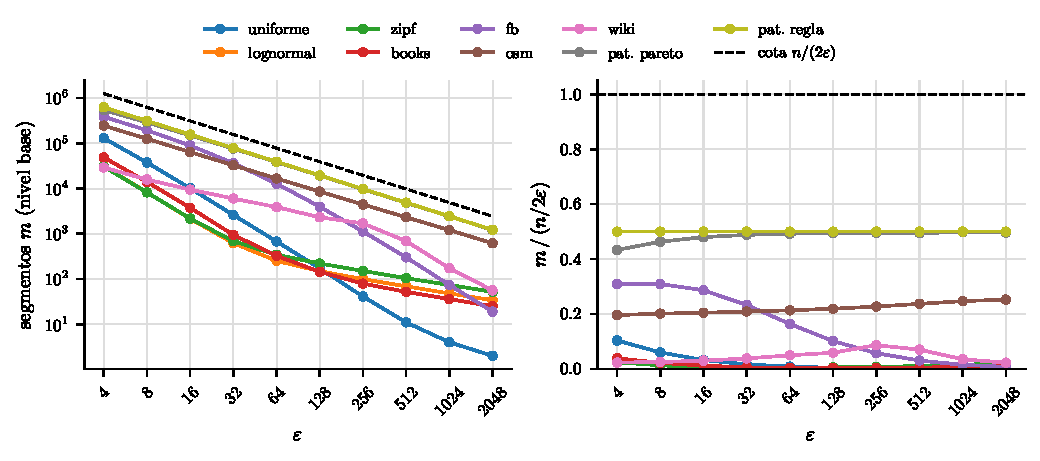
\includegraphics[width=\textwidth]{figuras/segmentos.pdf}
\caption{Izquierda: segmentos del nivel base $m$ según $\varepsilon$, con la cota
$n/(2\varepsilon)$ en línea discontinua. Derecha: $m$ dividido por la cota.}
\label{fig:segmentos}
\end{figure}

\begin{table}[htbp]
\centering\small
\caption{Tamaño del PGM-index con $n=10^7$ y $\varepsilon=64$.}
\label{tab:segmentos}
\begin{tabular}{@{}llrcr@{}}
\toprule
Conjunto & Tipo & Segmentos $m$ & Niveles & Tamaño \\
\midrule
\tabinput{tablas/segmentos.tex}
\bottomrule
\end{tabular}
\end{table}

En todos los conjuntos y para todo $\varepsilon$ se cumple la cota $m\le n/(2\varepsilon)$
(Figura~\ref{fig:segmentos}). En los datos regulares, $m$ queda muy por debajo de ella: con
$\varepsilon=64$, books indexa $10^7$ llaves con 326 segmentos, que ocupan 5\,KB
(Tabla~\ref{tab:segmentos}). Los datos reales más difíciles son osm, fb y friendster, con cerca del
20\,\% de la cota. Los patológicos pareto y regla llegan a la mitad de la cota, que es el peor caso
que observamos. En cambio, loggap, que parece irregular, resulta fácil.

En los datos regulares, $m$ cae más rápido que $1/\varepsilon$ cuando $\varepsilon$ va de 8 a 64,
como predice $m=O(n/\varepsilon^c)$ con $c>1$~\cite{ferragina2020icml}. En osm, wiki y los
patológicos de cola pesada, en cambio, cae a la misma velocidad que $1/\varepsilon$. La recursión
deja índices de 1 a 5 niveles, y construir uno de $10^7$ llaves toma menos de 200\,ms.

\subsection{P2. ¿Cómo influye $\varepsilon$ en el espacio y el tiempo?}

\begin{figure}[htbp]
\centering
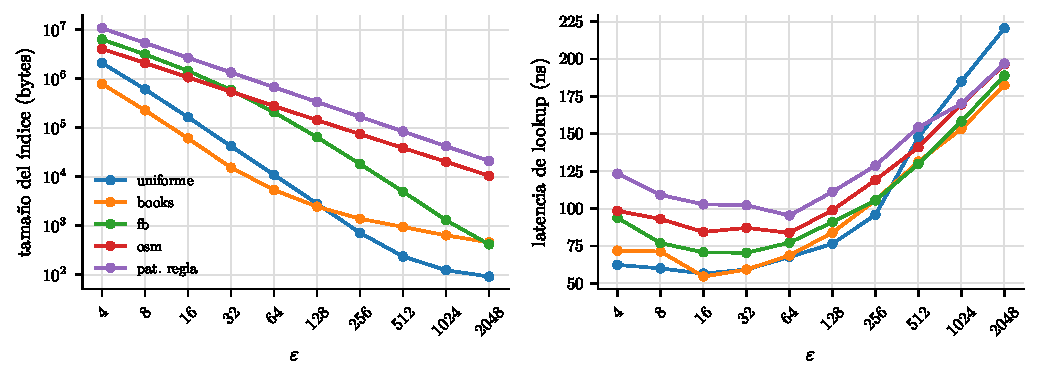
\includegraphics[width=\textwidth]{figuras/epsilon.pdf}
\caption{Efecto de $\varepsilon$ con $n=10^7$: tamaño del índice (izquierda) y tiempo por
consulta (derecha).}
\label{fig:epsilon}
\end{figure}

Al subir $\varepsilon$, el espacio cae varios órdenes de magnitud, pero el tiempo no baja
igual: tiene un mínimo entre $\varepsilon=16$ y $64$ (Figura~\ref{fig:epsilon}). Con
$\varepsilon$ grande domina la búsqueda binaria final sobre la ventana de $2\varepsilon$
llaves, y con $\varepsilon=2048$ el PGM ya no mejora a la búsqueda binaria sobre todo el arreglo
(183 a 221\,ns frente a unos 160\,ns). Con $\varepsilon$ muy pequeño el índice crece y gana niveles sin que la consulta mejore.
En la práctica, un $\varepsilon$ entre 16 y 64 es un buen punto de operación.

\subsection{P3. ¿Cuándo gana frente al B$^+$ tree y la búsqueda binaria?}

\begin{figure}[htbp]
\centering
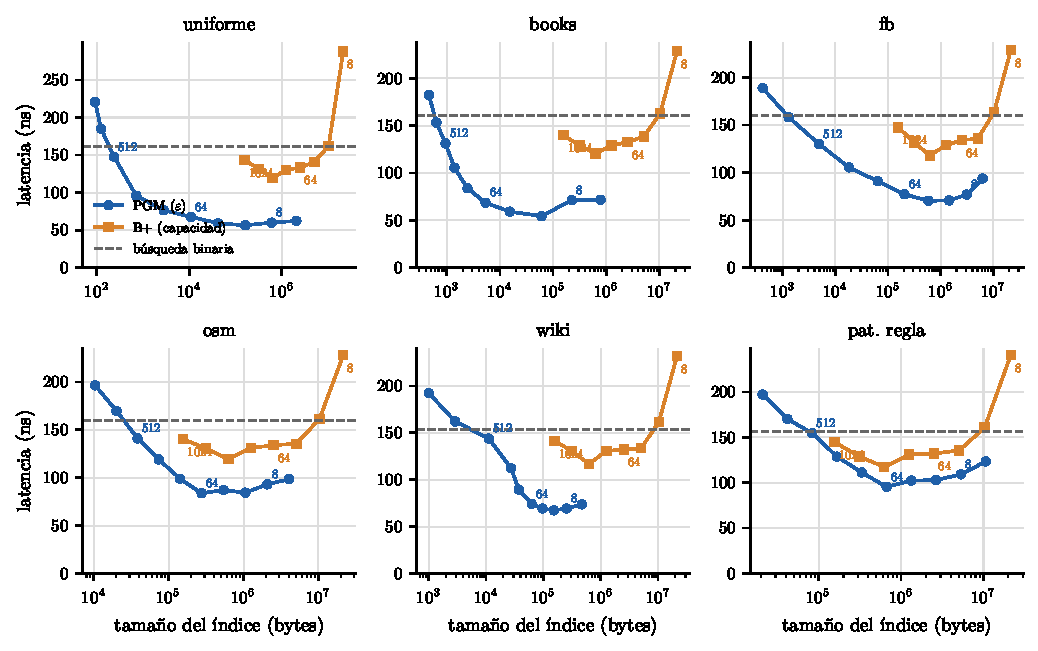
\includegraphics[width=0.85\textwidth]{figuras/pareto.pdf}
\caption{Espacio contra tiempo con $n=10^7$. Cada punto del PGM corresponde a un $\varepsilon$ y cada
punto del B$^+$ a una capacidad de nodo. Más abajo y a la izquierda es mejor.}
\label{fig:pareto}
\end{figure}

\begin{table}[htbp]
\centering\small
\caption{PGM ($\varepsilon=64$), B$^+$ (capacidad 64) y búsqueda binaria con $n=10^7$. El tiempo
es la mediana en ns por consulta.}
\label{tab:comparacion}
\begin{tabular}{@{}lrrrrrr@{}}
\toprule
& \multicolumn{3}{c}{Tiempo (ns)} & \multicolumn{3}{c}{Tamaño del índice} \\
\cmidrule(lr){2-4}\cmidrule(l){5-7}
Conjunto & Binaria & PGM & B$^+$ & PGM & B$^+$ & B$^+$/PGM \\
\midrule
\tabinput{tablas/comparacion.tex}
\bottomrule
\end{tabular}
\end{table}

Con $n=10^7$, el PGM es más rápido y más pequeño que el B$^+$ en los 14 conjuntos
(Figura~\ref{fig:pareto} y Tabla~\ref{tab:comparacion}). Responde en unos 60 a 100\,ns,
frente a unos 130 a 160\,ns del B$^+$ y 150 a 200\,ns de la búsqueda binaria, es decir,
entre 1,4 y 2,3 veces más rápido que el B$^+$ y entre 1,6 y 2,9 veces más rápido que la binaria,
alrededor de dos veces en la mayoría de los conjuntos. En espacio, el B$^+$ ocupa cientos de veces más en los datos
regulares. La ventaja se reduce en los datos más irregulares: en pareto y regla el B$^+$ ocupa
solo 4 veces más, y el mejor PGM es solo 1,2 a 1,3 veces más rápido que el mejor B$^+$.

\begin{figure}[htbp]
\centering
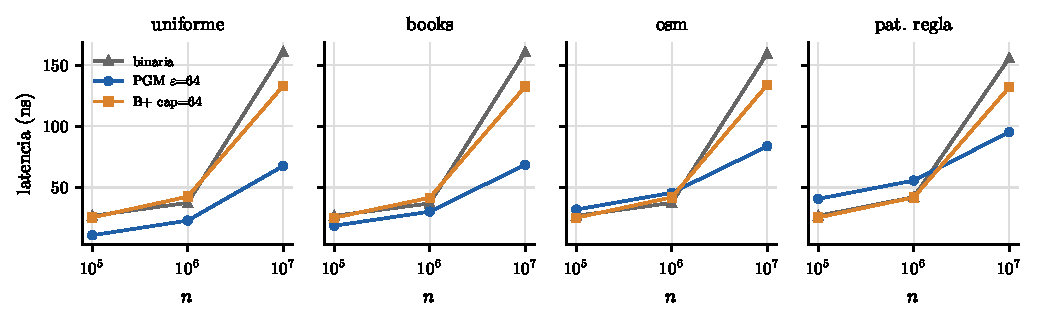
\includegraphics[width=0.85\textwidth]{figuras/tamanos.pdf}
\caption{Tiempo por consulta según $n$, con $\varepsilon=64$ y capacidad 64.}
\label{fig:tamanos}
\end{figure}

El tamaño del arreglo decide cuánto gana el PGM (Figura~\ref{fig:tamanos}). Con $n=10^5$ las
tres estructuras tardan unos 25 a 30\,ns: el PGM gana en los datos regulares,
pero pierde en osm, wiki, zipf, pareto y regla. Con $n=10^7$ las llaves ocupan 80\,MB: la búsqueda
binaria y el B$^+$ dan más pasos sobre el arreglo, mientras que el PGM solo busca dentro de la
ventana final. Ahí el PGM gana en todos los
conjuntos.

\subsection{Versiones dinámicas}
\label{sec:res-dyn}

\begin{figure}[htbp]
\centering
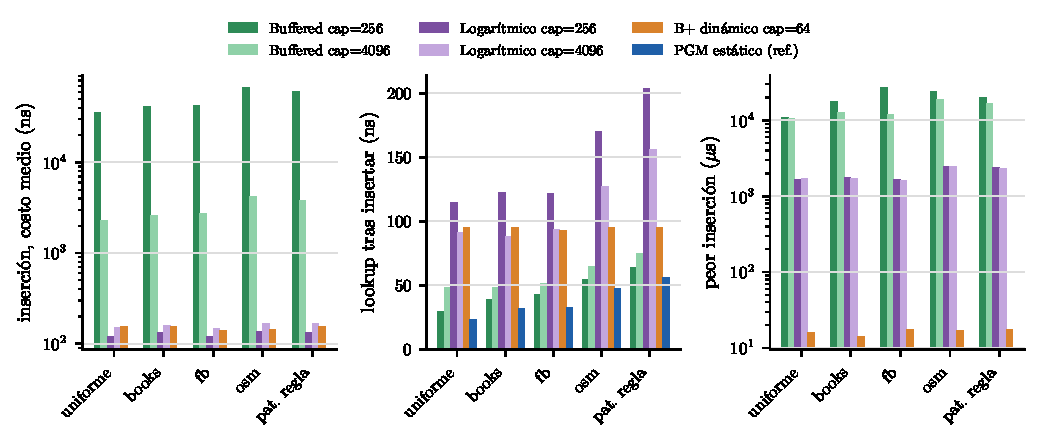
\includegraphics[width=\textwidth]{figuras/dinamicos.pdf}
\caption{Base de $10^6$ llaves más $2\times10^5$ inserciones: costo medio por inserción, tiempo de
búsqueda al terminar e inserción más lenta.}
\label{fig:dinamicos}
\end{figure}

Las dos variantes muestran el compromiso esperado (Figura~\ref{fig:dinamicos}).
\texttt{BufferedPGM} busca algo más lento que el estático (entre 1,3 y 2 veces), y cada
reconstrucción recorre toda la base. Por eso inserta en decenas de microsegundos con buffer 256 y
en unos pocos con buffer 4096, y tiene pausas de decenas de milisegundos.
\texttt{LogarithmicPGM} inserta en 120 a 170\,ns, a la par del B$^+$ dinámico (140 a 155\,ns), y a
cambio busca entre 2 y 4 veces más lento que el estático porque consulta varios niveles. Ambas ocupan casi la mitad de memoria que
el B$^+$ dinámico.


\section{Conclusiones}
\label{sec:conclusiones}

En el parcial nos propusimos implementar el PGM-index estático y compararlo con un B$^+$ tree y
con búsqueda binaria. Implementamos el PLA óptimo, el índice recursivo y los dos B$^+$, y los
medimos sobre 14 conjuntos de datos. Sobre la compacidad (P1), la cota $m\le n/(2\varepsilon)$ se
cumplió siempre. Con datos regulares el índice ocupa unos pocos KB para diez millones de llaves;
solo los casos patológicos de cola pesada llegan a la mitad de la cota. Sobre $\varepsilon$ (P2),
el espacio baja varios órdenes de magnitud al aumentarlo, pero el tiempo es mínimo entre
$\varepsilon=16$ y 64. Con valores mayores domina la búsqueda final, y con valores menores el
índice crece sin que la consulta mejore.

Sobre la ventaja práctica (P3), con arreglos grandes ($n=10^7$) el PGM responde unas dos veces
más rápido que el B$^+$ y que la búsqueda binaria, y ocupa cientos de veces menos que el B$^+$ en
los datos regulares. La ventaja se reduce cuando las llaves tienen saltos de cola pesada, porque
$m$ se acerca a la cota, y cuando el arreglo es chico ($n=10^5$). Además de lo
propuesto, implementamos dos versiones dinámicas del índice. La de buffer busca algo más lento
que el estático y conviene solo si las escrituras son raras. La logarítmica inserta a la par del
B$^+$ dinámico, a cambio de búsquedas varias veces más lentas que las del estático.


\small
\begin{thebibliography}{99}
\setlength{\itemsep}{0pt}

\bibitem{ferragina2020pgm}
P. Ferragina y G. Vinciguerra.
\emph{The PGM-index: a fully-dynamic compressed learned index with provable worst-case
bounds}. PVLDB 13(8): 1162--1175, 2020.

\bibitem{ferragina2019arxiv}
P. Ferragina y G. Vinciguerra.
\emph{The PGM-index: a multicriteria, compressed and learned approach to data indexing}.
arXiv:1910.06169, 2019.

\bibitem{kraska2018}
T. Kraska, A. Beutel, E. H. Chi, J. Dean y N. Polyzotis.
\emph{The Case for Learned Index Structures}. ACM SIGMOD, 489--504, 2018.

\bibitem{galakatos2019}
A. Galakatos, M. Markovitch, C. Binnig, R. Fonseca y T. Kraska.
\emph{FITing-Tree: A Data-aware Index Structure}. ACM SIGMOD, 1189--1206, 2019.

\bibitem{orourke1981}
J. O'Rourke.
\emph{An on-line algorithm for fitting straight lines between data ranges}.
Communications of the ACM, 24(9): 574--578, 1981.

\bibitem{xie2014}
Q. Xie, C. Pang, X. Zhou, X. Zhang y K. Deng.
\emph{Maximum error-bounded piecewise linear representation for online stream
approximation}. The VLDB Journal, 23(6): 915--937, 2014.

\bibitem{ferragina2020icml}
P. Ferragina, F. Lillo y G. Vinciguerra.
\emph{Why Are Learned Indexes So Effective?} ICML, PMLR 119: 3123--3132, 2020.
Versión extendida en Theoretical Computer Science 871: 107--120, 2021.

\bibitem{kipf2020}
A. Kipf, R. Marcus, A. van Renen, M. Stoian, A. Kemper, T. Kraska y T. Neumann.
\emph{RadixSpline: A Single-Pass Learned Index}. aiDM@SIGMOD, 2020.

\bibitem{ding2020}
J. Ding et al.
\emph{ALEX: An Updatable Adaptive Learned Index}. ACM SIGMOD, 969--984, 2020.

\bibitem{marcus2020}
R. Marcus, A. Kipf, A. van Renen, M. Stoian, S. Misra, A. Kemper, T. Neumann y T. Kraska.
\emph{Benchmarking Learned Indexes}. PVLDB 14(1): 1--13, 2020.

\bibitem{tsur2025}
E. Gæde, I. van der Hoog, E. Rotenberg y T. Stordalen.
\emph{Dynamic Indexing Through Learned Indices with Worst-case Guarantees}.
arXiv:2503.05007, 2025.

\end{thebibliography}



\end{document}
